\documentclass[aspectratio=169]{beamer}
\usepackage{subfigure}
% \usepackage{hyperref}
\usepackage[T1]{fontenc}
\usepackage{latexsym,amsmath,xcolor,multicol,booktabs,calligra}
\usepackage{graphicx,pstricks,listings,stackengine}
\usepackage{bm}

\usefonttheme[onlymath]{serif}
\usetheme{Madrid}

\title{Dynamic Uploading Scheduling in mmWave-Based Sensor Networks via Mobile Blocker Detection}
\subtitle{}
\author{
	Yifei~Sun{\textsuperscript\textdagger}{\textsuperscript\textdaggerdbl},
	~Bojie~Lv{\textsuperscript\textdagger},
	~Rui~Wang{\textsuperscript\textdagger},
	~Haisheng~Tan{\textsuperscript\textsection},
	~and~Francis~C.~M.~Lau{\textsuperscript\textdaggerdbl}
}
\institute[{\textsuperscript\textdagger}SUSTech, {\textsuperscript\textdaggerdbl}HKU, and {\textsuperscript\textsection}USTC]{
	{\textsuperscript\textdagger}Southern University of Science and Technology (SUSTech), Shenzhen, China \\
	{\textsuperscript\textdaggerdbl}The University of Hong Kong (HKU), Hong Kong, China \\
	{\textsuperscript\textsection}University of Science and Technology of China (USTC), Hefei, China}
\date{Dec. 20, 2023}
\usepackage{myslidesty} % this line must be placed here to work

\def\cmd#1{\texttt{\color{red}\footnotesize $\backslash$#1}}
\def\env#1{\texttt{\color{blue}\footnotesize #1}}
\definecolor{deepblue}{rgb}{0,0,0.5}
\definecolor{deepred}{rgb}{0.6,0,0}
\definecolor{deepgreen}{rgb}{0,0.5,0}
\definecolor{halfgray}{gray}{0.55}

\lstset{
    basicstyle=\ttfamily\small,
    keywordstyle=\bfseries\color{deepblue},
    emphstyle=\ttfamily\color{deepred},    % Custom highlighting style
    stringstyle=\color{deepgreen},
    numbers=left,
    numberstyle=\small\color{halfgray},
    rulesepcolor=\color{red!20!green!20!blue!20},
    frame=shadowbox,
}

\begin{document}
\begin{frame}
    \titlepage
\end{frame}

% \begin{frame}
% 	\tableofcontents[sectionstyle=show, subsectionstyle=show/shaded/hide, subsubsectionstyle=show/shaded/hide]
% \end{frame}

\section{Introduction}
\begin{frame}{Introduction}{Motivation}
    \begin{enumerate}
        \item The vulnerability of mmWave communication to link blockage postpones real-time communications, and thus results in outdated Age of Information (AoI) in Wireless Sensor Networks (WSNs).
        \item Fortunately, with wireless sensing technologies, the locations of signal reflectors (e.g., walls), the real-time position and motion pattern of an environmental blocker (e.g., a human body) can be detected to predict future wireless channels [1][2].
        \item As a result, future AoI degradation arising from link blockage can be forecast. Although we can not prevent the coming link blockage, future AoI outdatedness can be mitigated by taking action in advance. For example, the server prefer to sample and collect the status information from the sensor more frequently just before its link blockage.
    \end{enumerate}
    \vspace{10pt}
    \scriptsize
    [1] Y. Sun, et al., ``An Indoor Environment Sensing and Localization System via mmwave Phased Array,'' JCIN, 2022.
    
    [2] C. Yu, Y. Sun, et al., ``mmAlert: mmWave Link Blockage Prediction via Passive Sensing,'' IEEE WCL, 2023.
\end{frame}

\section{System Model}
\begin{frame}{System Model}{Network Description}
    \small
    We consider a mmWave-based wireless monitoring system consisting of one server connected with the base station (BS) and $K$ sensors in an indoor space with a mobile blocker.
    \normalsize

    \begin{minipage}[t]{0.5\linewidth}
        \begin{itemize}[<+->]
            \item<1-> \textbf{Sampling and uploading.} \only<1>{The sensors measure the status of physical process (e.g., photos) and upload the sample by transmitter via mmWave uplink channel. The server collects the received samples and maintains the latest sample. }
            \item<2-> \textbf{AoI-aware.} \only<2>{The AoI of a sample is defined as the time elapsed since it is generated at the sensor.}
            \item<3-> \textbf{Blocker-aware.} \only<3>{It is assumed that the real-time position and motion pattern (position transitions) of the blocker can be detected via wireless sensing technologies.}
        \end{itemize}
    \end{minipage}
    \hspace{0.01\linewidth}
    \begin{minipage}[t]{0.45\linewidth}
        \begin{figure}
            \centering
            \includegraphics[width=\textwidth]{fig/network_model_v2.pdf}
        \end{figure}
    \end{minipage}
\end{frame}

\begin{frame}{System Model}{Network Description}
    \begin{itemize}
        \item \textbf{Discretized time.} The uplink transmission time is organized by physical-layer frames with constant duration, where the channel state information (CSI) is assumed to be quasi-static in one frame.
        \item \textbf{Discretized space.} The locations of the indoor space are quantized into grids with indexes.
        \item It is assumed that the mobility of the blocker follows a time-invariant Markov chain, with the following transition probabilities,
        \begin{align*}
            \Pr\big[l_{t+1}^{\mathrm{B}}\!=\!\ell^{\prime}\big|l_{t}^{\mathrm{B}}\!=\!\ell\big]=\big[\mathbf{P}^{\mathrm{B}}\big]_{\ell,\ell^{\prime}},\ \forall{t},\ \forall \ell,\ell^{\prime}\in\mathbb{L},
        \end{align*}
        where $\mathbf{P}^{\mathrm{B}}\in\mathbb{R}^{|\mathbb{L}|\times|\mathbb{L}|}$ denotes the transition matrix of the blocker's mobility.
    \end{itemize}
\end{frame}

\begin{frame}{System Model}{Channel Model}
    We consider the geometric channel model with at most $M$ NLoS paths and one LoS path from each sensor to the BS. Hence, the channel matrix $\mathbf{H}_{t,k}\!\in\!\mathbb{C}^{N_{\mathrm{R}}\times N_{\mathrm{T}}}$ from the $k$-th sensor to the BS in the $t$-th frame can be written as
    \begin{align*}
        \label{eqn:H_tk}
        \mathbf{H}_{t,k}
        =
        \sum_{i\in\mathcal{M}}
        \underbrace{B_{t,k,i}(l_{t}^{\mathrm{B}})}_{
            \substack{\text{blockage}\\\text{indicator}}}
        \underbrace{\alpha_{t,k,i}}_{
            \substack{\text{complex}\\\text{gain}}}
        \underbrace{
            \mathbf{a}_{\mathrm{R}}(\phi_{k,i})
            \mathbf{a}_{\mathrm{T}}^{\mathsf{H}}(\theta_{k,i})}_{
                \substack{\text{array response}\\\text{w.r.t. AoA/AoD}}}.
    \end{align*}
    The human blocker is modeled as a disk with radius $r_{\mathrm{B}}$, and hence, given $l_{t}^{\mathrm{B}}$, the blockage indicator $B_{t,k,i}$ can be determined in a geometric way.

    The path loss of the LoS path is usually much smaller than that of the NLoS paths.
    Therefore, the uplink transmission suffers from significant degradation when the LoS path is blocked.
\end{frame}

\begin{frame}{System Model}{Channel Model}
    \small
    Given the transmission power at the sensor, the uplink capacity of the $k$-th sensor in the $t$-th frame after precoding and combining can be expressed by
    \begin{align*}
        R_{t,k}
        \triangleq
        W\log_{2}\Bigg(1+p_{t,k}\underbrace{\frac{\big|\mathbf{w}_{t,k}^{\mathsf{H}}\mathbf{H}_{t,k}\mathbf{f}_{t,k}\big|^{2}}{\|\mathbf{w}_{t,k}\|^{2}N_{0}W}}_{\textrm{Baseband gain $Y_{t,k}$}}\Bigg).
    \end{align*}

    Time-Division Multiple Access (TDMA) is adopted in each frame.
    The transmission time allocated to the $k$-th sensor, $\tau_{t,k}$ is constrained by
    \begin{align*}
        &
        \textstyle{
        \sum_{k\in\mathcal{K}}\tau_{t,k}=T_{\mathrm{F}},\ \forall{t},
        }
        \\
        &
        0\leq\tau_{t,k}\leq T_{\mathrm{F}},\ \forall{t,k}\in\mathcal{K}.
    \end{align*}
    With the packet size $N_{\mathrm{b}}$, the number of packets transimitted in a frame can be expressed by 
    \begin{align*}
        D_{t,k}=\big\lfloor\frac{R_{t,k}\tau_{t,k}}{N_{\mathrm{b}}}\big\rfloor.
    \end{align*}
\end{frame}


\begin{frame}{System Model}{Queuing and AoI Model}
    \footnotesize
    The data volume of each sample generated by the $k$-th sensor consists of $L_{k}$ packets, which may not be completely uploaded in one frame. Let $s_{t,k}\!\in\!\{0,1\}$ be the sampling action. 
    Since each sensor only transmits data packets of the latest sample, the queue dynamics of the $k$-th sensor (in terms of packets) is given by
    \begin{minipage}[t]{0.55\linewidth}
        \vspace{-10pt}
        \begin{align*}
            Q_{t+1,k}=
            \begin{cases}
                (Q_{t,k}\!-\!D_{t,k})^{+}, & s_{t,k}=0 \\
                L_{k}-D_{t,k},         & s_{t,k}=1 \\
            \end{cases}
        \end{align*}
        
        The AoI dynamics at the $k$-th sensor is given by
        \begin{align*}
            A_{t+1,k}^{\mathrm{s}}
            \!=\!
            \begin{cases}
                \min\{A_{t,k}^{\mathrm{s}}+1,A_{\mathrm{max}}\}, & s_{t,k}=0 \\
                1,                                               & s_{t,k}=1
            \end{cases}
        \end{align*}

        The AoI dynamics for the $k$-th sensor at the server is given by
        \begin{align*}
            A_{t+1,k}^{\mathrm{d}}
            \!=\!
            \begin{cases}
                \min\{A_{t,k}^{\mathrm{s}}\!+\!1,A_{\mathrm{max}}\}\!,
                &
                (Q_{t,k}\!-\!D_{t,k})^{+}\!=\!0 \\
                \min\{A_{t,k}^{\mathrm{d}}\!+\!1,A_{\mathrm{max}}\}\!,
                &
                \mathrm{otherwise}
            \end{cases}
        \end{align*}
    \end{minipage}
    \hspace{0.01\linewidth}
    \begin{minipage}[t]{0.40\linewidth}
        \begin{figure}
            \centering
            \includegraphics[width=\textwidth]{fig/network_model_v2.pdf}
        \end{figure}
    \end{minipage}
\end{frame}

\section{Problem Formulation}
\begin{frame}{Problem Formulation}{Infinite-horizon MDP}
    To formulate the problem as an infinite-horizon MDP, we shall define:
    \begin{block}{System State}
        At the beginning of the $t$-th frame, the \textbf{global system state} is defined by $\mathcal{S}_{t}\!\triangleq\!(l_{t}^{\mathrm{B}},\mathcal{Y}_{t},\mathcal{Q}_{t},\mathcal{A}_{t}^{\mathrm{s}},\mathcal{A}_{t}^{\mathrm{d}})$ consisting of blocker location, and baseband channel power gains, queue lengths, AoIs at the sensors, AoIs for the sensors at the server.
    \end{block}

    \begin{block}{Action and Policy}
        The \textbf{global scheduling action} is defined by $\mathbf{a}_{t}\!\triangleq\!(s_{t,k},\tau_{t,k},p_{t,k})_{k\in\mathcal{K}}$, including the sampling decision, and uplink transmission time and power.
        Hence, the \textbf{scheduling policy} is a mapping from the system state to the scheduling actions, $\Omega(\mathcal{S}_{t})=\mathbf{a}_{t}$.
    \end{block}
\end{frame}

\begin{frame}{Problem Formulation}{Infinite-horizon MDP}
    \begin{block}{Per-frame Cost}
        In the $t$-th frame, the \textbf{per-frame cost} is defined by
        \begin{align*}
            g(\mathcal{S}_{t},\Omega(\mathcal{S}_{t}))
            =
            \sum\nolimits_{k\in\mathcal{K}}\big[
                \underbrace{A_{t,k}^{\mathrm{d}}}_{\substack{\text{AoI at}\\\text{the server}}}
                +
                w_{\mathrm{P}}(
                    \underbrace{s_{t,k}C^{\mathrm{s}}}_{\substack{\text{sampling}\\\text{energy}}}
                    +
                    \underbrace{\tau_{t,k}p_{t,k}}_{\substack{\text{transmission}\\\text{energy}}}
                )
                +
                w_{\mathrm{Q}}
                \underbrace{\mathbb{I}[A_{t,k}^{\mathrm{d}}=A_{\mathrm{max}}]}_{\substack{\text{AoI outdatedness}\\\text{penalty}}}
                \big],
        \end{align*}
        where $w_{\mathrm{P}}$ and $w_{\mathrm{Q}}$ denote the weights for energy consumption and AoI outdatedness penalty, respectively.
    \end{block}
\end{frame}


\begin{frame}{Problem Formulation}{Infinite-horizon MDP}
    \begin{block}{Infinite-horizon MDP}
        As a result, the joint sampling and uploading optimization can be formulated as the infinite-horizon MDP with discounted cost,
        \begin{align*}
            \mathsf{P1}:\
            \Omega^{\star}
            =
            \mathop{\arg\min}_{\Omega}\
            & \lim_{T\rightarrow\infty}\left[\mathbb{E}_{\mathcal{Y},\mathcal{L}^{\mathrm{B}}}\sum\nolimits_{t=1}^{T}\gamma^{t\!-\!1}g_{t}(\mathcal{S}_{t},\Omega(\mathcal{S}_{t}))\Big|\mathcal{S}_{1}\right]\nonumber                                                                        \\
            \mathrm{s.t.}\
            & p_{t,k}\leq P_{\mathrm{max}},\ \forall{t},{k}\in\mathcal{K},  \\
            & \sum\nolimits_{k\in\mathcal{K}}\tau_{t,k}=T_{\mathrm{F}},\ \forall{t}, \\
            & 0\leq\tau_{t,k}\leq T_{\mathrm{F}},\ \forall{t,k}\in\mathcal{K}.
        \end{align*}
    \end{block}
\end{frame}

\begin{frame}{Problem Formulation}{Infinite-horizon MDP}
    The Bellman's equations of the above MDP are
    \begin{align*}
        W(\mathcal{S})
        =
         &
        \textstyle{
        \min_{\Omega(\mathcal{S})}\big[g\big(\mathcal{S},\Omega(\mathcal{S})\big)
        }
        \nonumber
        \\
         &
        +
        \textstyle{
            \gamma\sum_{\mathcal{S}^{\prime}}W(\mathcal{S}^{\prime})\Pr[\mathcal{S}^{\prime}|\mathcal{S},\Omega(\mathcal{S})]\big],\
        }
        \forall\mathcal{S},
    \end{align*}

    Although conventional approaches such as policy iteration (PI) and value iteration (VI) can be used to find the optimal scheduling policy by recursion of the Bellman equation, they suffer from the \textit{curse of dimensionality}: due to the huge system state space, the evaluation of value function is prohibitive.
\end{frame}

\section{Proposed Solution}
\begin{frame}{Proposed Solution}{}
    \begin{minipage}[t]{0.45\linewidth}
        \begin{figure}
            \centering
            \includegraphics[width=\textwidth]{fig/framework_slides_v2.pdf}
        \end{figure}
    \end{minipage}
    \hspace{0.01\linewidth}
    \begin{minipage}[t]{0.5\linewidth}
        \small 
        The proposed suboptimal solution achieves a good balance between complexity and performance.
        \begin{itemize}
            \item \textbf{Low Complexity.}
            \begin{enumerate}
                \item Analytically expressed and decoupled value function of reference policy.
                \item One-step policy improvement instead of iteration.
                \item Alternative optimization for the decoupled actions during policy improvement.
            \end{enumerate}
            \item \textbf{Performance Guarantee.} {The performance of the proposed policy is lower-bounded by a roughly-good reference policy.}
        \end{itemize}
    \end{minipage}
\end{frame}

\section{Simulation Results}
\begin{frame}{Simulation Results}{Benchmarks}
    We compare the proposed policies with three benchmarks. For fair comparison, all the benchmarks adopt the same sampling policy and transmission power as the reference policy of our proposed framework, while the time allocation is:
    \begin{itemize}
        \item \textbf{BM 1} (Reference Policy) The transmission time allocation of each sensor is proportional to the corresponding data volume of sample at each sensor, i.e., $
		\tau_{t,k}\!=\!T_{\mathrm{F}}L_{k}/\sum_{k^{\prime}\!\in\!\mathcal{K}}L_{k^{\prime}}
	$.
        \item \textbf{BM 2} (Largest-AoI First) The sensor with the largest AoI at the server, i.e., $\mathop{\arg\max}_{k}A_{t,k}^{\mathrm{d}}$, is scheduled for transmission sequentially, until transmission time of the frame is used up.
        \item \textbf{BM 3} (Dynamic Backpressure) The sensor with the largest product of buffer length and uplink capacity, i.e., $\mathop{\arg\max}_{k}Q_{t,k}R_{t,k}$,  is scheduled for transmission sequentially, until transmission time of the frame is used up.
    \end{itemize}
\end{frame}

\begin{frame}{Simulation Results}{A Deeper Look at How it Works}
    \begin{minipage}[t]{0.45\linewidth}
        We consider a 20m$\times$20m square room with $8$ sensors and the mobility of the human blocker follows a modified random walk.
        \begin{figure}
            \centering
            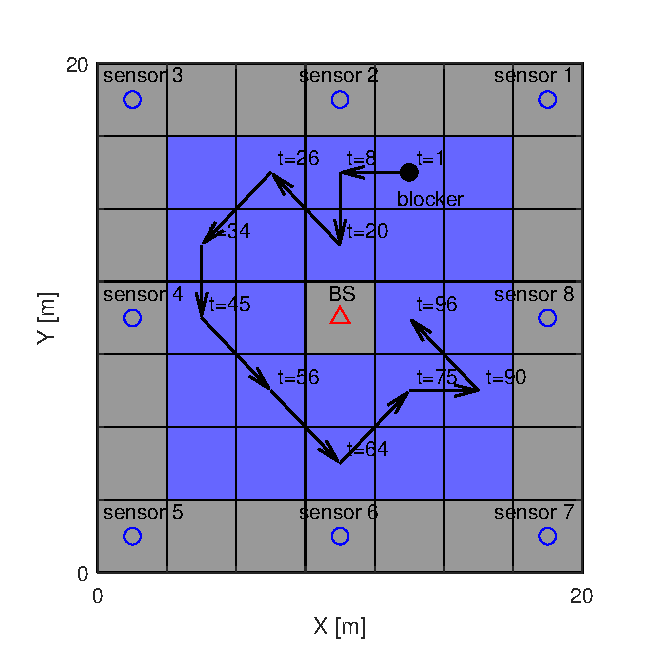
\includegraphics[width=0.6\textwidth]{fig/layout.eps}
        \end{figure}
    \end{minipage}
    \hspace{0.01\linewidth}
    \begin{minipage}[t]{0.45\linewidth}
        The insights on blockage-predictive scheduling of the proposed policy can be obtained, which shows the dynamics of the AoI at the $4$-th sensor and the corresponding AoI at the server.
        % It can be observed from the trajectory of the blocker for this trace, the LoS path between the BS and the $4$-th sensor is blocked since the $45$-th frame.
        % Compared with BM1, the proposed policy can detect future channel degradation, and keep the AoIs at the $4$-th sensor and the BS at a low level before the $45$-th frame, which reduces the time duration with outdated AoI at the server.
        \begin{figure}[htb]
            \centering
            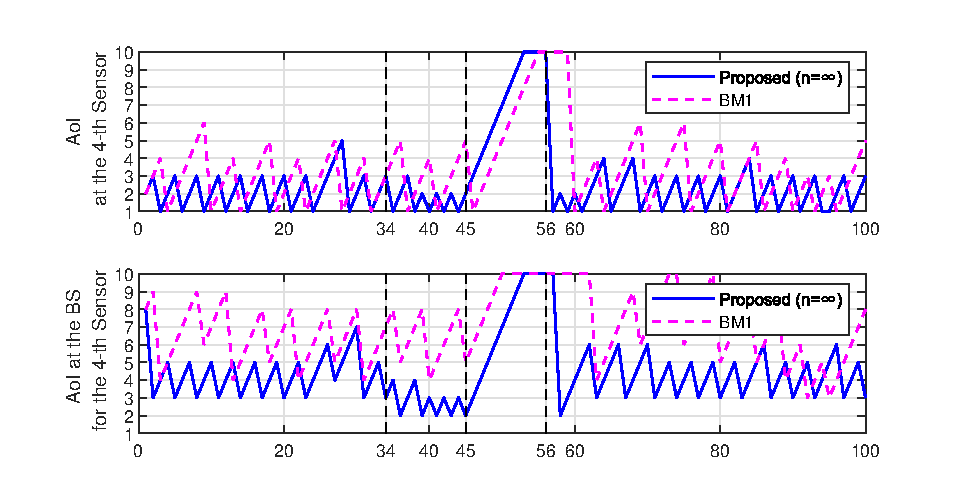
\includegraphics[width=0.85\linewidth]{fig/insight.eps}
        \end{figure}
    \end{minipage}
\end{frame}

\begin{frame}{Simulation Results}{Comparison with Benchmarks}
    Our proposed scheme can converge after only a few iterations and reduce the average per-frame cost by $13.5\%$--$49.6\%$ compared with the benchmarks.
    \begin{minipage}[t]{0.45\linewidth}
        \begin{figure}
            \centering
            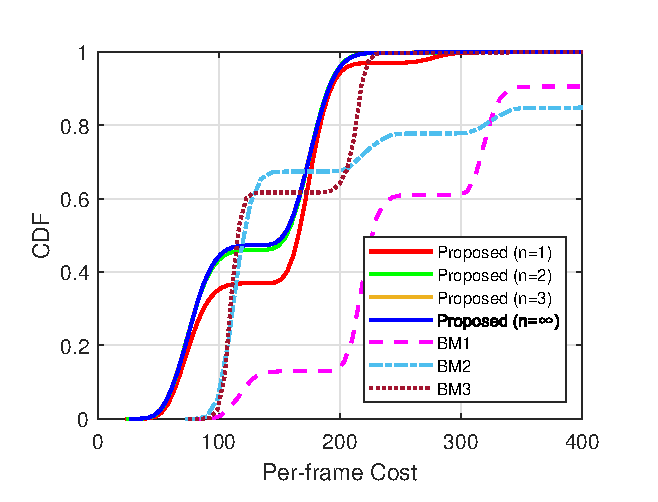
\includegraphics[width=0.8\linewidth]{fig/CDF.eps}
        \end{figure}
    \end{minipage}
    \hspace{0.01\linewidth}
    \begin{minipage}[t]{0.45\linewidth}
        \begin{figure}[htb]
            \centering
            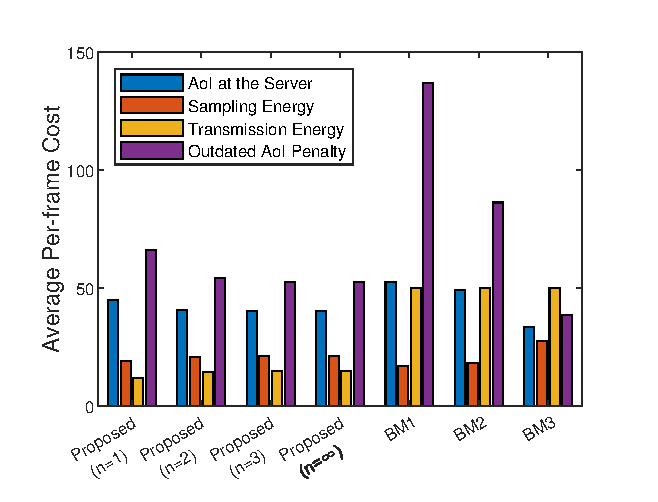
\includegraphics[width=0.8\linewidth]{fig/barplot.eps}
        \end{figure}
    \end{minipage}
\end{frame}

\begin{frame}{Simulation Results}{Impact of the Number of Sensors}
    Our proposed scheme shows the better performance compared to the benchmarks with robustness against the number of sensors.
    \begin{figure}[htb]
        \centering
        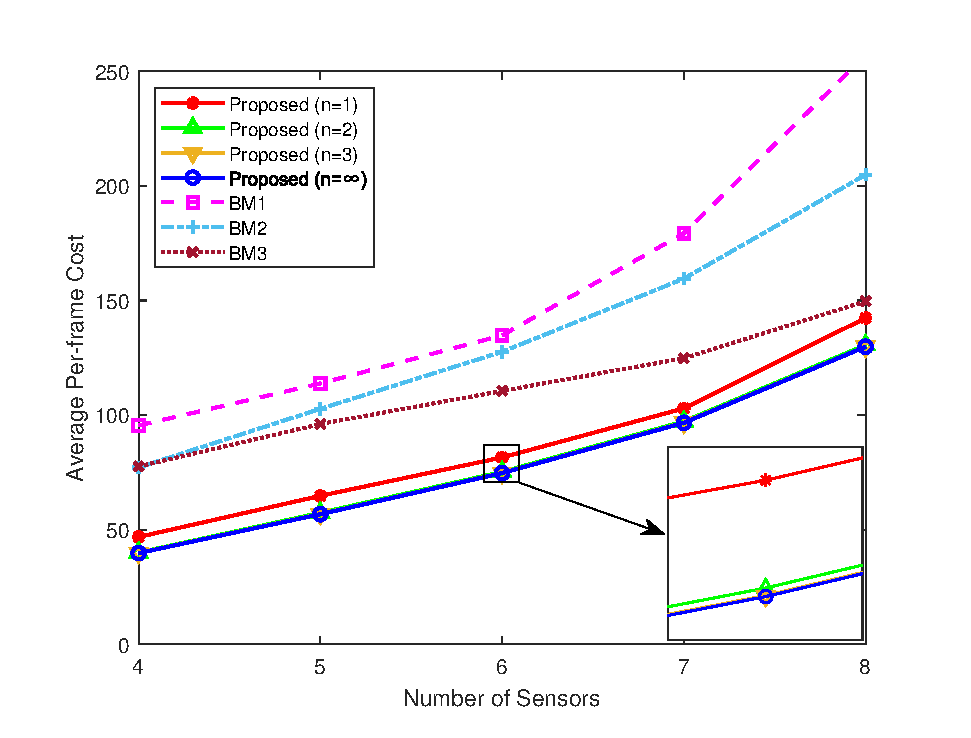
\includegraphics[width=0.4\linewidth]{fig/SenAnaK.eps}
    \end{figure}
\end{frame}

\section{Conclusion}
\begin{frame}{Conclusion}{}
    \begin{itemize}
        \item
              A predictive scheduling framework is provided for environment-aware transmission scheduling.
              In the proposed MDP formulation, the future AoI degradation due to potential link blockage is naturally considered in the current scheduling according to the Bellman's equations.
        \item
              We propose a low-complexity AMDP framework with a guarantee of the worst-case performance.
              Specifically, we first introduce a decoupling principle to design heuristic scheduling polices as the reference policy, whose average cost can be derived analytically.
              With the expression of the value function, the above policy iteration can be formulated analytically, whose optimization efficiency is significantly better than the conventional numerical search.
        \item
              Simulations show that compared with several heuristic benchmarks, our proposed policy, benefiting from the awareness of the link blockage, can reduce the average cost with a high performance gain.
    \end{itemize}
\end{frame}

\end{document}